\documentclass[a4paper]{article}

\setlength{\parindent}{0pt}
\setlength{\parskip}{1em}

\pagestyle{headings}

\usepackage{amssymb}
\usepackage{amsmath}
\usepackage{amsthm}
\usepackage{mathtools}
\usepackage{graphicx}
\usepackage{hyperref}
\usepackage{color}
\usepackage{microtype}
\usepackage{tikz}
\usepackage{pgfplots}
\usepackage{pgfplotstable}

\newcommand{\N}{\mathbb{N}}
\newcommand{\Q}{\mathbb{Q}}
\newcommand{\Z}{\mathbb{Z}}
\newcommand{\R}{\mathbb{R}}
\newcommand{\C}{\mathbb{C}}
\newcommand{\D}{\mathcal{D}}
\renewcommand{\S}{\mathcal{S}}
\renewcommand{\P}{\mathbb{P}}
\newcommand{\F}{\mathbb{F}}
\newcommand{\E}{\mathbb{E}}
\newcommand{\bra}{\langle}
\newcommand{\ket}{\rangle}


\graphicspath{{Image/}}

\hypersetup{
    colorlinks=true,
    linktoc=all,
    linkcolor=blue
}

\theoremstyle{definition}
\newtheorem*{axiom}{Axiom}
\newtheorem*{claim}{Claim}
\newtheorem*{conv}{Convention}
\newtheorem*{coro}{Corollary}
\newtheorem*{defi}{Definition}
\newtheorem*{eg}{Example}
\newtheorem*{lemma}{Lemma}
\newtheorem*{notation}{Notation}
\newtheorem*{prob}{Problem}
\newtheorem*{post}{Postulate}
\newtheorem*{prop}{Proposition}
\newtheorem*{rem}{Remark}
\newtheorem*{thm}{Theorem}

\DeclareMathOperator{\vdiv}{div}
\DeclareMathOperator{\grad}{grad}
\DeclareMathOperator{\curl}{curl}
\DeclareMathOperator{\Ann}{Ann}
\DeclareMathOperator{\Fit}{Fit}
\DeclareMathOperator{\Diag}{Diag}
\DeclareMathOperator{\tr}{tr}
\DeclareMathOperator{\im}{im}
\DeclareMathOperator{\Mat}{Mat}
\DeclareMathOperator{\Log}{Log}
\DeclareMathOperator{\Isom}{Isom}
\DeclareMathOperator{\Mesh}{Mesh}
\DeclareMathOperator{\Sym}{Sym}
\DeclareMathOperator{\Aut}{Aut}
\DeclareMathOperator{\cosech}{cosech}
\DeclareMathOperator{\Card}{Card}
\DeclareMathOperator{\Gal}{Gal}


\setcounter{section}{-1}

\begin{document}

\title{Representation Theory}

\maketitle

\newpage

\tableofcontents

\newpage

\section{Introduction}
Representaiton theory is the theory of how \emph{groups} act as groups of linear transformations on \emph{vector spaces}. 

Here the groups are either \emph{finite}, or \emph{compact topological groups} (infinite), for example, $SU(n)$ and $O(n)$. The vector spaces we conside are finite dimensional, and usually over $\C$. Actions are \emph{linear} (see below).

Some books: James-Liebeck (CUP); Alperin-Bell (Springer); Charles Thomas, \emph{Representations of finite and Lie groups}; Onlne notes: SM, Teleman; P.Webb \emph{A course in finite group representation theory} (CUP); Charlie Curtis, \emph{Pioneers of representation theory} (history).

\newpage

\section{Group actions}

Throughout this course, if not specified otherwise:\\
$\bullet$ $F$ is a field, usually $\C$, $\R$ or $\Q$. When the field is one of these, we are discussing \emph{ordinary representation theory}. Sometimes $F=F_p$ or $\bar{F}_p$ (algebraic closure, see Galois Theory), in which case the theory is called \emph{modular representation theory};\\
$\bullet$ $V$ is a vector space over $F$, always finite dimensional;\\
$GL(V) =\{\theta : V \to V, \theta$ linear, invertible$\}$, i.e. $\det \theta \neq 0$.

Recall from Linear Algebra:\\
If $\dim_F V = n < \infty$, choose basis $e_1,...,e_n$ over $F$, so we can identify it with $F^n$. Then $\theta \in GL(V)$ corresponds to an $n \times n$ matrix $A_\theta = (a_{ij})$, where $\theta(e_j) = \sum_i a_{ij} e_i$. In fact, we have $A_\theta \in GL_n(F)$, the general linear group.

(1.1) $GL(V) \cong GL_n(F)$ as groups by $\theta \to A_\theta$ ($A_{\theta_1 \theta_2} = A_{\theta_1} A_{\theta_2}$ and bijection).\\
Choosing different basis gives different isomorphism to $GL_n(F)$, but:

(1.2) Matrices $A_1,A_2$ represent the same element of $GL(V)$ w.r.t different bases iff they are conjugate (similar), i.e. $\exists X \in GL_n(F)$ s.t. $A_2 =XA_1 X^{-1}$.

Recall that $\tr(A) = \sum_i a_{ii}$ where $A = (a_{ij})$, the \emph{trace} of $A$.

(1.3) $\tr(XAX^{-1}) = \tr(A)$, hence we can define $\tr(\theta) = \tr(A_{\theta_1})$ independent of basis.

(1.4) Let $\alpha \in GL(V)$ where $V$ in f.d. over $\C$, with $\alpha^m = \iota$ for some $m$ (here $\iota$ is the identity map). Then $\alpha$ is diagonalisable.

Recall $EndV$ is the set of all ilnear maps $V \to V$, e.g. $End(F^n) =M_n(F)$ some $n \times n$ matrices.

(1.5) \emph{Proposition.} Take $V$ f.d. over $\C$, $\alpha \in End(V)$. Then $\alpha$ is diagonalisable iff there exists a polynomial $f$ with distinct linear factors with $f(\alpha) = 0$. For example, in (1.4), where $\alpha^m = \iota$, we take $f = X^m - 1 = \prod_{j=0}^{m-1} (X-\omega^j)$ where $\omega = e^{2\pi i/m}$ is the ($m^{th}$) root of unity. In fact we have:

(1.4)* A finite family of commuting separately diagonalisable automorphisms of a $\C$-vector space can be simultaneously diagonalised (useful in abelian groups).

Recall from Group Theory:\\
(1.6) The symmetric group, $S_n = Sym(X)$ on the set $X = \{1,...,n\}$ is the set of all permutations of $X$. $|S_n| = n!$. The alternating group $A_n$ on $X$ is the set of products of an even number of transpositions (2-cycles). $|A_n| = \frac{n!}{2}$.

(1.7) Cyclic groups of order $m$: $C_m = <x:x^m = 1>$. For example, $(\Z/m\Z, +)$; also, the group of $m^{th}$ roots of unity in $\C$ (inside $GL_1(\C)$ = $\C^*$, the multiplicative group of $\C$). We also have the group of rotations, centre $O$ of regular $m-$gon in $\R^2$ (inside $GL_2(\R)$).

(1.8) Dihedral groups $D_{2m}$ of order $2m = <x,y: x^m = y^2 = 1, yxy^{-1} = x^{-1}>$. Think of this as the set of rotations and reflections preserving a regular $m$-gon.

(1.9) Quaternion group, $Q_8 = <x,y|x^4 = 1, y^2 = x^2, yxy^{-1} = x^{-1}>$ of order $8$. For example, in $GL_2(\C)$, put $i={{i\ 0} \choose {0 \ i}}, j = {{0 \ 1} \choose {-1 \ 0}}, k = {{0 \ i} \choose {i \ 0}}$, then $Q_8 = \{\pm I_2, \pm i, \pm j, \pm k\}$.

(1.10) The conjugacy class (ccls) of $g \in G$ is $\mathcal{C}_G(g) = \{xgx^{-1} : x \in G\}$. Then $|\mathcal{C}_G (g) | = |G:C_G(g)|$, where $C_G(g) = \{x \in G : xg = gx\}$, the centraliser of $g \in G$.

(1.11) Let $G$ be a group, $X$ be a set. $G$ acts on $X$ if there exists a map $\cdot: G \times X \to X$ by $(g,x) \to g\cdot x$ for $g \in G$, $x \in X$, s.t. $1 \cdot x = x$ for all $x \in X$, $(gh) \cdot x = g \cdot (h\cdot x)$ for all $g,h \in G, x \in X$.

(1.12) Given an action of $G$ on $X$, we obtain a homomorphism $\theta: G \to Sym(X)$, called the \emph{permutation representation} of $G$.
\begin{proof}
For $g \in G$, the function $\theta_g: X \to X$ by $x \to gx$ is a permutation on $X$, with inverse $\theta_{g^{-1}}$. Moreover, $\forall g_1,g_2 \in G$, $\theta_{g_1 g_2} = \theta_{g_1} \theta_{g_2}$ since $(g_1g_2) x = g_1(g_2 x)$ for $x \in X$.
\end{proof}

\newpage

\section{Basic Definitions}
\subsection{Representations}

Let $G$ be finite, $F$ be a field, usually $\C$.
\begin{defi} (2.1)\\
Let $V$ be a f.d. vector space over $F$. A (linear, in some books) \emph{representation} of $G$ on $V$ is a group homomorphism 
\begin{equation*}
\begin{aligned}
\rho = \rho_V: & G &\to GL(V)
\end{aligned}
\end{equation*}
Write $\rho_g$ for the image $\rho_V(g)$; so for each $g \in G$, $\rho_g \in GL(V)$, and $\rho_{g_1 g_2} = \rho_{g_1} \rho_{g_2}$, and $(\rho_g)^{-1} = \rho_{g^{-1}}$.\\
The \emph{dimension} (or \emph{degree}) of $\rho$ is $\dim_F V$.
\end{defi}

(2.2) Recall $\ker \rho \triangleleft G$ (kernel is a normal subgroup), and $G/\ker \rho \cong \rho(G) \leq GL(V)$ (1st isomorphism theorem). We say $\rho$ is \emph{faithful} if $\ker \rho = 1$.

An alternative (and equivalent) approach is to observe that a representation of $G$ on $V$ is "the same as" a \emph{linear action} of $G$:

\begin{defi} (2.3)\\
$G$ \emph{acts linearly} on $V$ if there exists a \emph{linear action}
\begin{equation*}
\begin{aligned}
G \times V &\to V\\
(g,v) &\to gv
\end{aligned}
\end{equation*}
By linear action we mean: (action) $(g_1 g_2) v = g_1(g_2 v)$, $1v=v$ $\forall g_1,g_2 \in G, v \in V$, and (linear) $g(v_1+v_2) = gv_1+gv_2$, $g(\lambda v) = \lambda gv$ $\forall g \in G, v_1,v_2 \in V, \lambda \in F$.\\
Now if $G$ acts linearly on $V$, the map
\begin{equation*}
\begin{aligned}
G &\to GL(V)\\
g &\to \rho_g
\end{aligned}
\end{equation*}
with $\rho_g:v \to gv$ is a representation of $G$. Conversely, given a representation $\rho: G \to GL(V)$, we have a linear action of $G$ on $V$ via $g \cdot v := \rho(g) v$ $\forall v \in V, g \in G$.
\end{defi}

(2.4) In (2.3) we also say that $V$ is a $G$-space or that $V$ is a $G$-module. In fact if we define the \emph{group algebra} $FG$, or $F[G]$, to be $\{ \sum \alpha_j g: \alpha_j \in F\}$ with natural addition and multiplication, then $V$ is actually a $FG$-module (in the sense from GRM).

(2.5) $R$ is a \emph{matrix representation} of $G$ of degree $n$ if $R$ is a homomorphism $G \to GL_n (F)$. Given representation $\rho:G \to GL(V)$ with $\dim_F V=n$, fix basis $B$; we get matrix representation
\begin{equation*}
\begin{aligned}
G &\to GL_n(F)\\
g &\to [\rho(g)]_B
\end{aligned}
\end{equation*}
Conversely, given matrix representation $R:G \to GL_n(F)$, we get representation
\begin{equation*}
\begin{aligned}
\rho: G &\to GL(F^n)\\
g &\to \rho_g
\end{aligned}
\end{equation*}
via $\rho_g(v) = R_g v$ where $R_g$ is the matrix of $g$.

\begin{eg} (2.6)\\
Given any group $G$, take $V=F$ the 1-dimensional space, and 
\begin{equation*}
\begin{aligned}
\rho:G &\to GL(F)\\
g &\to (id: F \to F)
\end{aligned}
\end{equation*}
is known as the trivial representation of $G$. So $\deg \rho = 1$ ($\dim_F F = 1$).
\end{eg}

\begin{eg} (2.7)\\
Let $G=C_4 = <x:x^4=1>$. Let $n=2$, and $F=\C$. Note that any $R:x \to X$ will determine $x^j \to X^j$ as it is a homomorphism, and also we need $X^4 = I$. So we can take $X$ to be diagonal matrix -- any such with diagonal entries a root to $x^4=1$, i.e. $\{\pm 1,\pm i\}$, or if $X$ is not diagonal then it will be similar to a diagonal matrix by (1.4) ($X^4=I$).
\end{eg}

\subsection{Equivalent representations}

\begin{defi} (2.8)\\
Fix $G,F$. Let $V,V'$ be $F$-spaces, and $\rho:G \to GL(V)$, $\rho': G \to GL(V')$ which are representations of $G$. The linear map $\phi: V \to V'$ is a $G$-homomorphism if $$\phi\rho(g) = \rho'(g)\phi \forall g \in G (*)$$ We can understand this more by the following diagram:

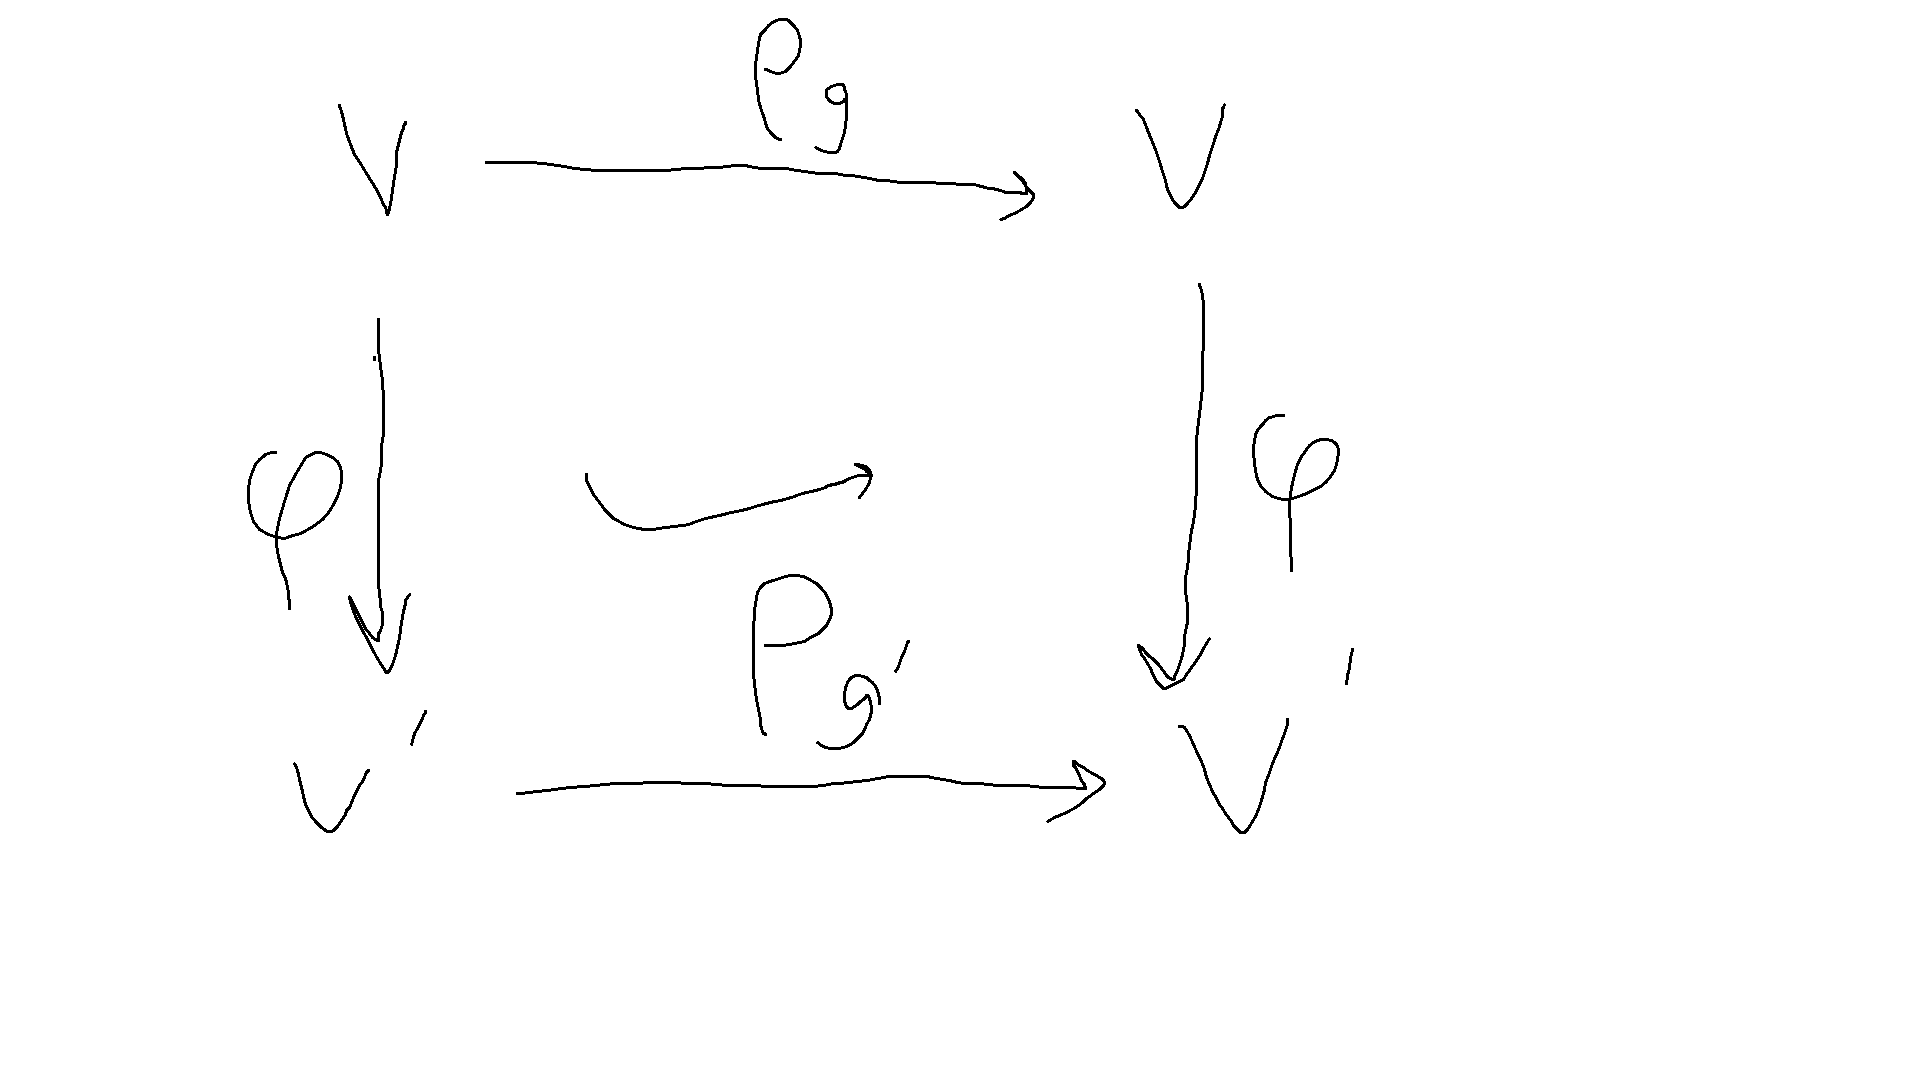
\includegraphics[scale=0.5]{image/Rep_01.png}

We say $\phi$ \emph{intertwines} $\rho,\rho'$. Write $Hom_G(V,V')$ for the $F$-space of all these.\\
$\phi$ is a $G$-isomorphism if it is also bijective; if such $\phi$ exists, $\rho,\rho'$ are isomorphic/equivalent representations. If $\phi$ is a $G$-isomorphism, we can write $(*)$ as $\rho' = \phi\rho\phi^{-1}$.
\end{defi}

\begin{lemma} (2.9)\\
The relation "being isomorphic" is an equivalent relation on the set of all representations of $G$ (over $F$).
\end{lemma}

\begin{rem} (2.10)\\
If $\rho,\rho'$ are isomorphic representations, they have the same dimension.

The converse may be false: $C_4$ has four non-isomorphic 1-dimensional representations: if $\omega = e^{2\pi i/4}$ then they are $\rho_j(x^i) = \omega^{ij}$ ($0 \leq i \leq 3$).
\end{rem}

\begin{rem} (2.11)\\
Given $G$, $V$ over $F$ of dimension $n$ and $\rho:G \to GL(V)$. Fix basis $B$ for $V$: we get a linear isomorphism 
\begin{equation*}
\begin{aligned}
\phi:V &\to F^n\\
v &\to [v]_B
\end{aligned}
\end{equation*}
and we get a representation $\rho': G \to GL(F^n)$ isomorphic to $\rho$:

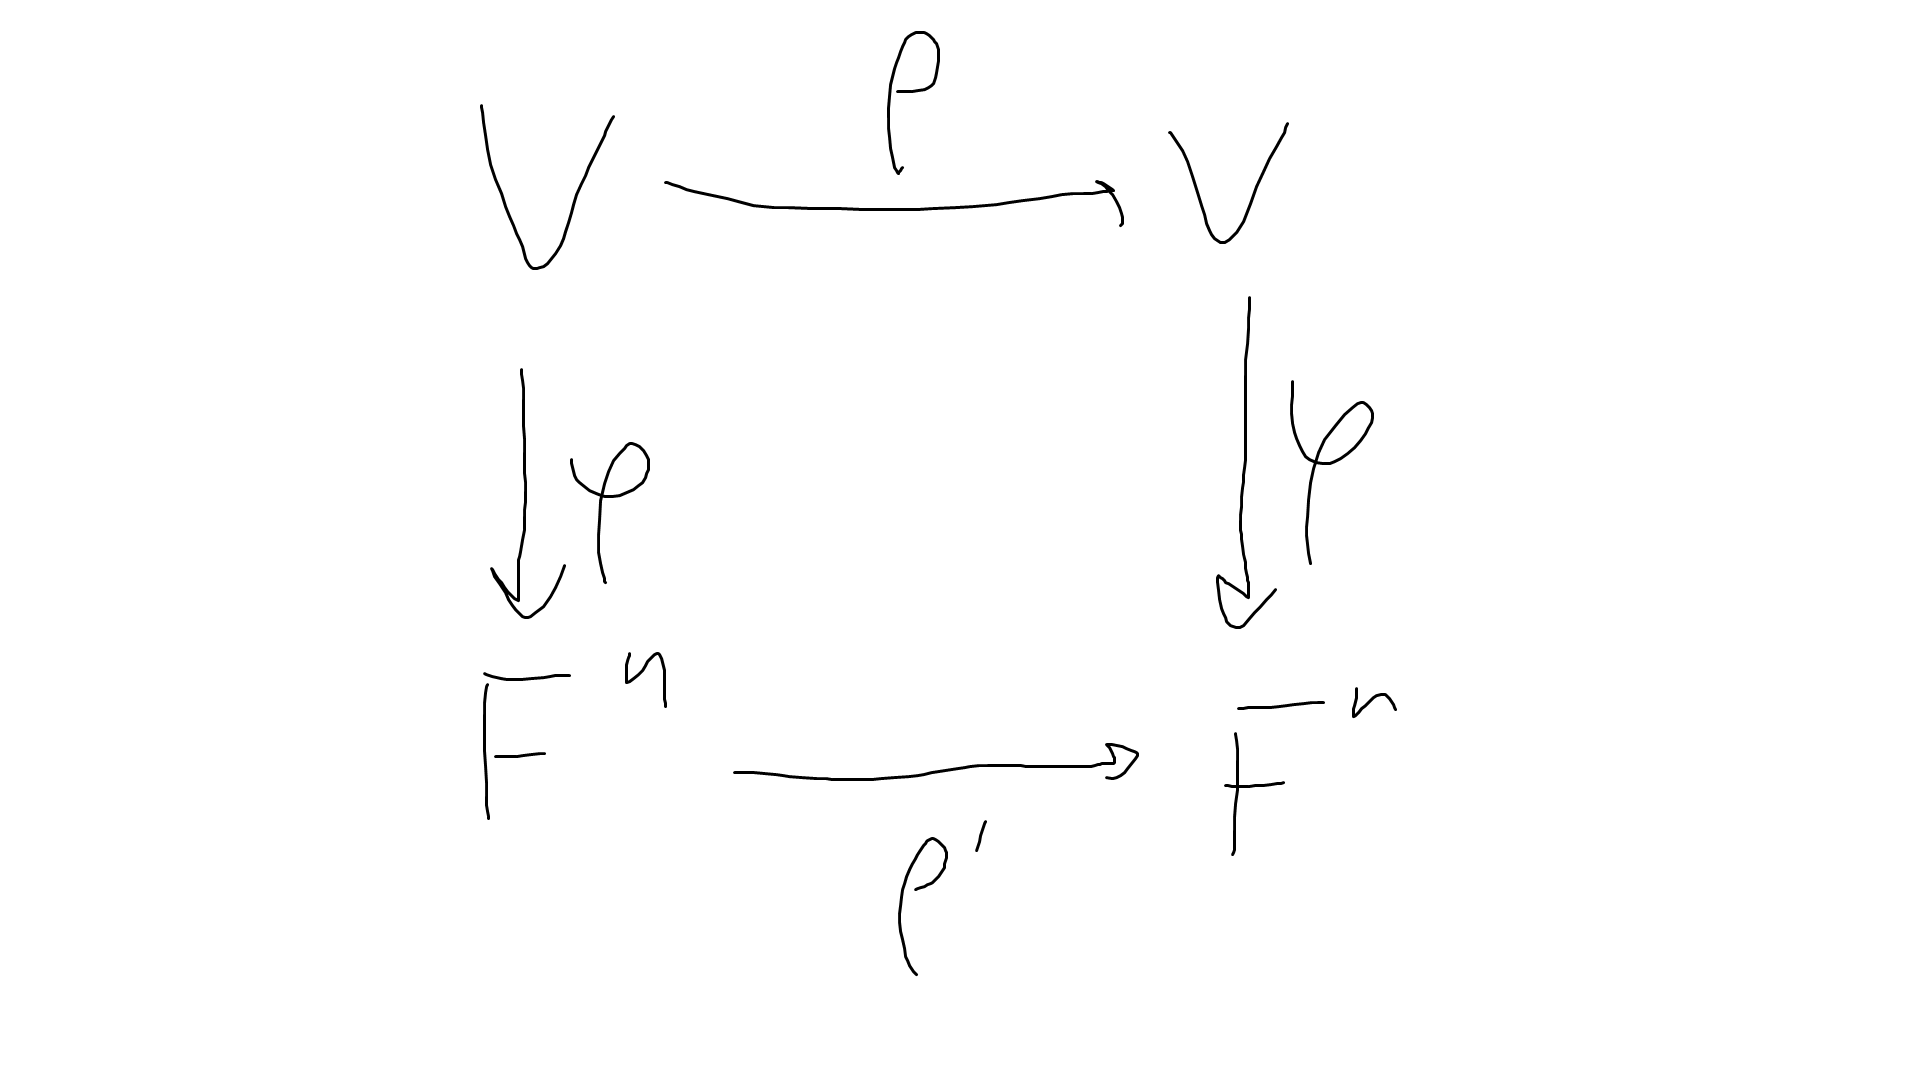
\includegraphics[scale=0.5]{image/Rep_02.png}
\end{rem}

(2.12) In terms of matrix representations, we have
\begin{equation*}
\begin{aligned}
R: G &\to GL_n(F),\\
R':G &\to GL_n(F)
\end{aligned}
\end{equation*}
are ($G$)-isomorphic or equivalent if there exists a nonsingular matrix $X \in GL_n(F)$ with $R'(g) = XR(g)X^{-1}$ $\forall g \in G$.

In terms of linear $G$-actions, the actions of $G$ on $V$,$V'$ are $G$-isomorphic if there exists isomorphisms $\phi:V \to V'$ such that $g:\phi(v) = \phi(gv)$ $\forall v \in V,g \in G$.

\subsection{Subrepresentations}
\begin{defi} (2.13)\\
Let $\rho:G \to GL(V)$ be a representation of $G$. We say $W \leq V$ is a $G$-subspace if it's a subspace and it is $\rho(G)$-invariant, i.e. $\rho_g(W) \leq W \forall g \in G$. Obviously $\{0\}$ and $V$ are $G$-subspaces, however.\\
$\rho$ is \emph{irreducible/simple} representation if there are no proper $G$-subspaces.
\end{defi}

\begin{eg} (2.14)\\
Any $1$-dimensional representation of $G$ is irreducible, but not conversely, e.g. $D_8$ has $2$-dimensional $\C$-irreducible representation.
\end{eg}

(2.15) In definition (2.13), if $W$ is a $G$-subspace, then the corresponding map
\begin{equation*}
\begin{aligned}
G &\to GL(W)\\
g &\to \rho(g)|_W
\end{aligned}
\end{equation*}
is a representation of $G$, a \emph{subrepresentation} of $\rho$.

\begin{lemma} (2.16)\\
In definition (2.13), given $\rho:G \to GL(V)$, if $W$ is a $G$-subspace of $V$ and if $B=\{v_1,...,v_n\}$ is a basis containing basis $B_1 = \{v_1,...,v_m\}$ of $W$ ($0<m<n$) then the matrix of $\rho(g)$ w.r.t. $B$ has block upper triangular form as the graph below, for each $g \in G$.
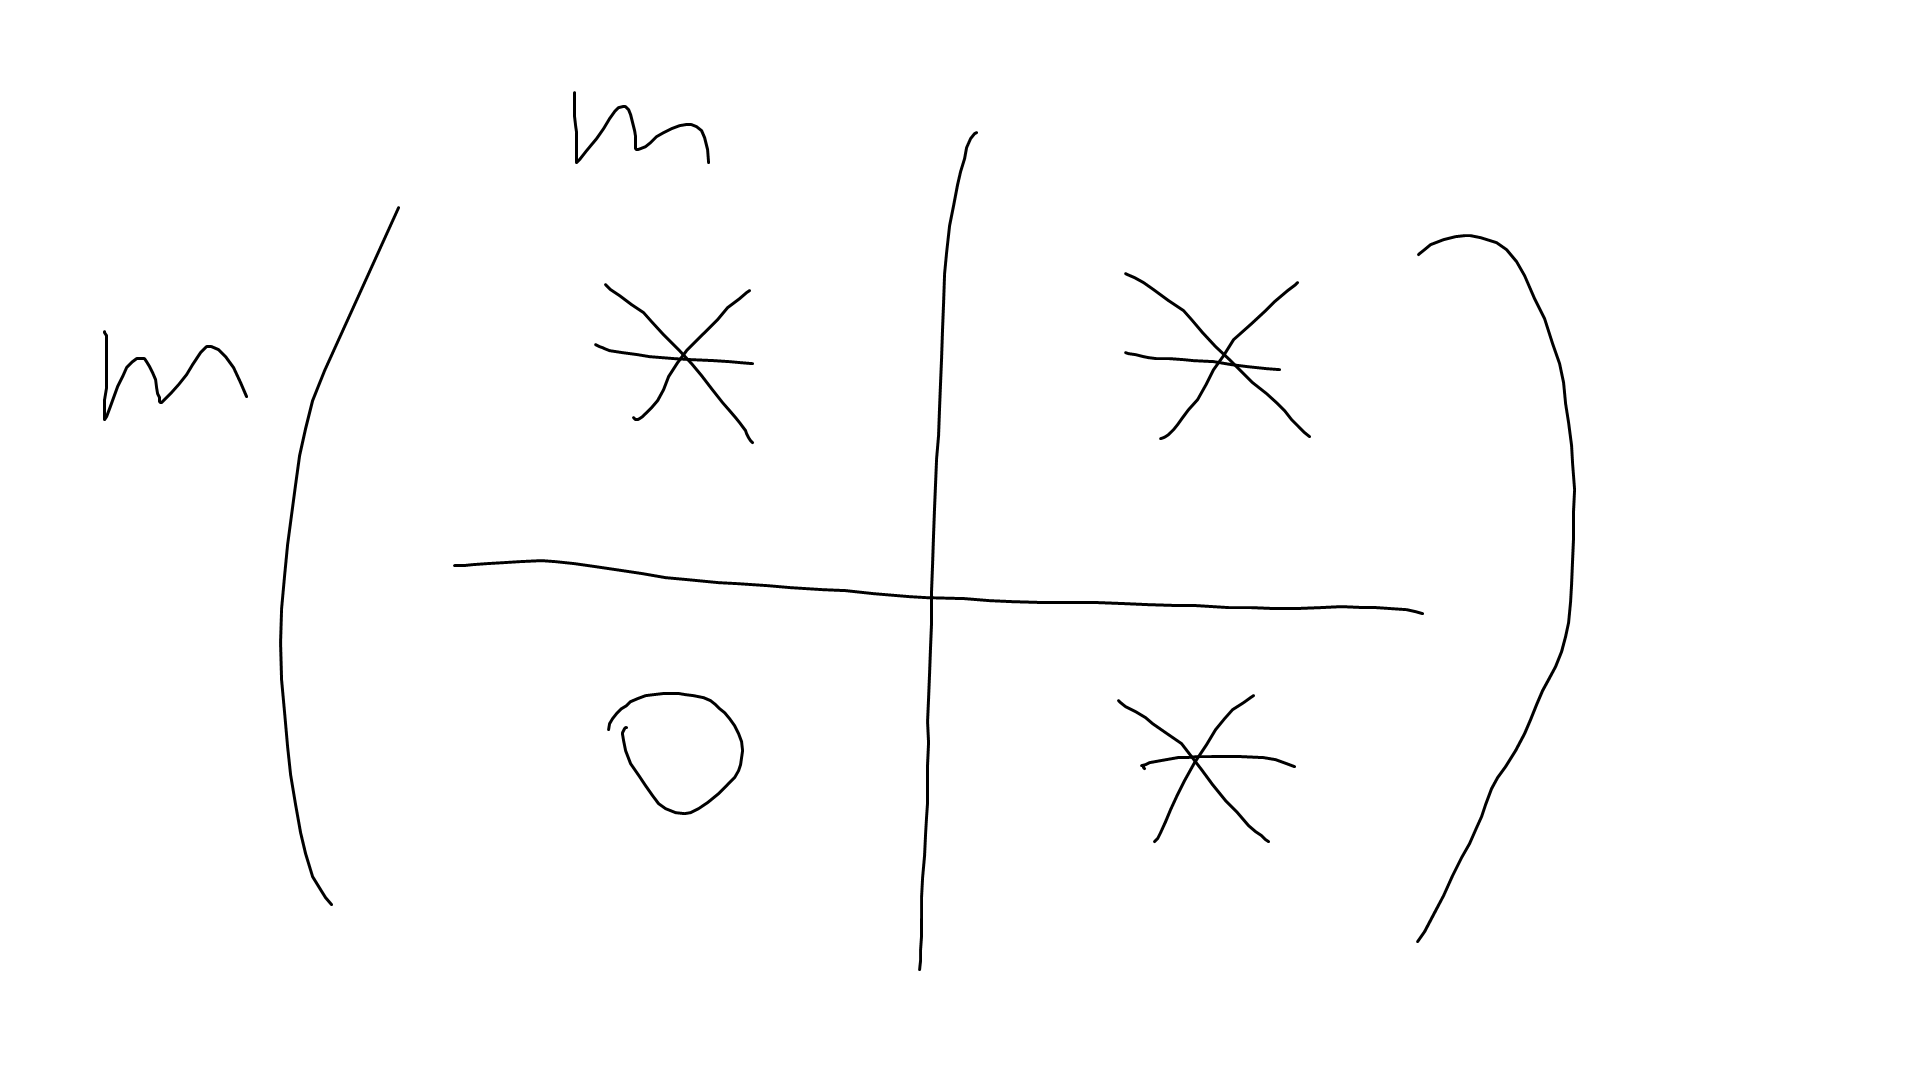
\includegraphics[scale=0.5]{image/Rep_03.png}
\end{lemma}

\begin{eg} (2.17)\\
(i) The irreducible representations of $C_4=\bra x:x^4=1\ket$ are all $1$-dimensional and four of these are $x\to i,x \to -1, x \to -i, x \to 1$. In general, $C_m=\bra x:x^m=1\ket$ has precisely $m$ irreducible complex representations, all of dimension 1. In fact, all complex irreducible representations of a finite abelian group are $1$-dimensional (use (1.4)* or see (4.4) below).\\
(ii) $G=D_6$: any irreducible $C$-representation has dimension $\leq 2$.\\
Let $\rho:G \to GL(V)$ be irreducible $G$-representation. Let $r,s$ be rotation and reflection in $D_6$ respectively. Let $V$ be eigenvector of $\rho(r)$. So $\rho(r) v = \lambda v$ for some $\lambda \neq 0$. Let $W=span\{v,\rho(s)v\} \leq V$. Since $\rho(s)\rho(s)v = v$ and $\rho(r)\rho(s) v = \rho(s)\rho(r)^{-1} v = \lambda^{-1} \rho(s) v$, both of which are in $W$; so $W$ is $G$-invariant, i.e. a $G$-subspace. Since $V$ is irreducible, $W=V$.
\end{eg}

\begin{defi} (2.18)\\
We say at $\rho:G \to GL(V)$ is \emph{decomposable} if there are proper $G$-invariant subspaces $U,W$ with $V = U \oplus W$. Say $\rho$ is direct sum $\rho_U \oplus \rho_W$. If no such decomposition exists, we say that $\rho$ is \emph{indecomposable}.
\end{defi}

\begin{lemma} (2.19)\\
Suppose $\rho:G \to GL(V)$ is decomposable with $G$-invariant decomposition $V=U \oplus W$. If $B$ is a basis $\{\underbrace{u_1,...,u_k}_{B_1}, \underbrace{w_1,...,w_l}_{B_2}\}$ of $V$ consisting of basis of $U$ and basis of $W$, then w.r.t. $B$, $\rho(g)_B$ is a block diagonal matrix $\forall g\in G$ as 
\begin{equation*}
\begin{aligned}
\rho(g)_B = \begin{pmatrix}
[\rho_W(g)]_{B_1} & 0\\
0 & [\rho_W(g)]_{B_2}
\end{pmatrix}
\end{aligned}
\end{equation*}
\end{lemma}

\begin{defi} (2.20)\\
If $\rho:G \to GL(V)$, $\rho':G \to GL(V')$, the \emph{direct sum} of $\rho,\rho'$ is $$\rho \oplus \rho':G \to GL(V \oplus V')$$ where $\rho \oplus \rho'(g) (v_1+v_2) = \rho(g)v_1 + \rho'(g) v_2$, a \emph{block diagonal action}. For matrix representations $R:G \to GL_n(F)$, $R':G \to GL_{n'} (F)$, define $R \oplus R': G \to GL_{n+n'}(F)$:
\begin{equation*}
\begin{aligned}
g \to \begin{pmatrix}
R(g) & 0\\
0 & R'(g)
\end{pmatrix}
\end{aligned}
\end{equation*}
\end{defi}

\newpage
\section{Complete reducibility and Maschke's theorem}
\begin{defi} (3.1)\\
A representation $\rho:G \to GL(V)$ is \emph{completely reducible}, or \emph{semisimple}, if it is a direct sum of irreducible representations. Evidently, irreducible implies completely reducible (lol).
\end{defi}

\begin{rem} (3.2)\\
(1) The converse is false;\\
(2) See sheet 1 Q3: $\C$-representation of $\Z$ is not completely reducible and also representation of $C_p$ over $\F_p$ is not c.r..

Fron now on, take $G$ finite and $char\ F =0$.
\end{rem}

\begin{thm} (3.3)\\
Every f.d. representation $V$ of a finite group over a field of char $0$ is completely reducible, i.e. $$V \cong V_1 \oplus ... \oplus V_r$$is a direct sum of representations, each $V_i$ irreducible.
\end{thm}

It is enough to prove:

\begin{thm} (3.4 Maschke's theorem, 1899)\\
Let $G$ be finite, $\rho:G \to GL(V)$ a f.d. representation, $char\ F = 0$. If $W$ is a $G$-subspace of $V$, then there exists a $G$-subspace $U$ of $V$ s.t. $V = W \oplus U$, a direct sum of $G$-subspaces.
\begin{proof} (1)\\
Let $W'$ be any \emph{vector subspace} complement of $W$ in $V$, i.e. $V=W \oplus W'$ as vector spaces, and $W \cap W'=0$. Let $q:V \to W$ be th projection of $V$ onto $W$ along $W'$ ($\ker q = W'$), i.e. if $v=w+w'$ then $q(v) = w$. Define $$\bar{q} : v \to \frac{1}{|G|} \sum_{g \in G} g q(g^{-1}v)$$the 'average' of $q$ over $G$. Note that in order for $\frac{1}{|G|}$ to exists, we need $char\ F = 0$. It still works if $char\ F \nmid |G|$.\\
Claim (1): $\bar{q}:V \to W$: For $v \in V$, $g(q^{-1}v) \in W$ and $gW \leq W$;\\
Claim (2): $\bar{q}(w) = w$ for $w \in W$: $$\bar{q}(w) = \frac{1}{|G|} \sum_{g \in G} gq(g^{-1}w) = \frac{1}{|G|} \sum g(g^{-1}w) = \frac{1}{|G|} \sum w = w$$
So these two claims imply that $\bar{q}$ projects $V$ onto $W$.\\
Claim (3) If $h \in G$ then $h\bar{q}(v) = \bar{q}(hv)$ ($v \in V$):
\begin{equation*}
\begin{aligned}
h\bar{q}(v) &= h\frac{1}{|G|} \sum_g g \cdot q(g^{-1} v)\\
&= \frac{1}{|G|} \sum_g hgq(g^{-1} v)\\
&= \frac{1}{|G|} \sum (hg) q((hg)^{-1} hv)\\
&= \frac{1}{|G|} \sum_g gq(g^{-1}(hv))\\
&= \bar{q}(hv\\
&= \bar{q}(hv))
\end{aligned}
\end{equation*}
We'll then show that the kernel of this map is $G$-invariant, so this gives a $G$-summand on Thursday.

Let's now show $\ker \bar{q}$ is $G$-invariant. If $v \in \ker \bar{q}$, then $h\bar{q}(v) = 0 = \bar{q}(hv)$, so $hv \in \ker \bar{q}$. Thus $V = im \bar{q} \oplus \ker \bar{q} = W \oplus \ker \bar{q}$ is a $G$-subspace decomposition.

We can deduce (3.3) from (3.4) by induction on $\dim V$. If $\dim V = 0$ or $V$ is irreducible, then result is clear. Otherwise, $V$ has non-trivial $G$-invariant subspace, $W$. Then by (3.4), there exists $G$-invariant complement $U$ s.t. $V = U \oplus W$ as representations of $G$. But $\dim U, \dim W < \dim V$. So by induction they can be broken up into direct sum of irreducible subrepresentations.
\end{proof}

The second proof uses inner products, hence we need to take $F = \C$ and can be generalised to compact groups in section 15.\\
Recall, for $V$ a $\C$-space, $\bra,\ket$ is a \emph{Hermitian inner product} if\\
(a) $\bra w,v\ket =\overline{\bra v,w\ket}$ $\forall v,w$ (Hermitian);\\
(b) linear in RHS (sesquilinear);\\
(c) $\bra v,v\ket > 0$ iff $v \neq 0$ (positvie definite).

Additionally, $\bra,\ket$ is \emph{G-invariant} if \\
(d) $\bra gv,gw\ket = \bra v,w\ket$ $\forall v,w \in V, g \in G$.

Note if $W$ is $G$-invariant subspace of $V$, with $G$-invariant inner product, then $W^\perp$ is also $G$-invariant, and $V \oplus W^\perp$. For all $v \in W^\perp$, $g \in G$, we have to show that $gv \in W^\perp$. But $v \in W^\perp \iff \bra v,w\ket = 0 \forall w \in W$. Thus by (d), $\bra gv,gw\ket = 0$ $\forall g \in G \forall w \in W$. Hence $\bra gv,w'\ket = 0$ $\forall w' \in W$. Since we can choose $w=g^{-1}w' \in W$ by $G$-invariance of $W$. Thus $gv \in W^\perp$ since $g$ was arbitrary.

Hence if there is a $G$-invariant inner product on any $G$-space, we get another proof of Maschke's theorem:

(3.4*) (Weyl's unitary trick)\\
Let $\rho$ be a complex representation of the finite group $G$ on the $\C$-space $V$. Then there is a $G$-invariant Hermitian inner product on $V$.
\begin{rem}
Recall the \emph{unitary group} $U(V)$ on $V$: $\{f \in GL(V): (fu,fv) = (u,v) \forall u,v \in V\} = \{A \in GL_n(\C) : A \bar{A}^T = I\} (= U(n))$ by choosing orthonormal basis.\\
Sheet 1 Q.12: any finite subgroup of $GL_n(\C)$ is conjugate to a subgroup of $U(n)$.
\end{rem}

\begin{proof} (2)\\
There exist an inner product on $V$: take basis $e_1,...,e_n$ and define $(e_i,e_j) = \delta_{ij}$, extended sesquilinearly. Now
\begin{equation*}
\begin{aligned}
\bra v,w\ket := \frac{1}{|G|} \sum_{g \in G} (gv,gw)
\end{aligned}
\end{equation*}
we claim that $\bra,\ket$ is sesquilinear, positive definite and $G$-invariant: if $h \in G$, then
\begin{equation*}
\begin{aligned}
\bra hv,hw\ket = \frac{1}{|G|} \sum_{g \in G} ((gh)v,(gh)w)\\
&= \frac{1}{|G|} \sum_{g' \in G} (g'v, g'w)\\
&= \bra v,w\ket
\end{aligned}
\end{equation*}
for all $v,w \in V$.
\end{proof}
\end{thm}

\begin{defi} (3.5, the regular representation)\\
Recall \emph{group algebra} of $G$ is $F$-space $FG = span\{e_g:g \in G\}$. There is a linear $G$-action
\begin{equation*}
\begin{aligned}
h \in G, h \sum_{g \in G} a_g e_g = \sum_{g \in G} a_g e_{hg} (=\sum_{g' \in G} a_{h^{-1} g'} e_{g'})
\end{aligned}
\end{equation*}
$\rho_{reg}$ is the corresponding representation, the \emph{regular representation} of $G$. This is faithful of $\dim |G|$. $FG$ is the \emph{regular module}.
\end{defi}

\begin{prop}
Let $\rho$ be an irreducible representation of $G$ over a field of characteristic 0. Then $\rho$ is isomorphic to a subrepresentation of $\rho_{reg}$.
\begin{proof}
Take $\rho: G \in GL(V)$ irreducible and let $0 \neq v \in V$. Let $\theta : FG \to V$ by $\sum a_g e_g \to \sum a_g gv$. Check this is a $G$-homomorphism. Now $V$ is irreducible so $im\theta = V$ (since $im\theta$ is a $G$-subspace).

Also $\ker\theta$ is $G$-subspace of $FG$. Let $W$ be $G$-complement of $\ker \theta$ in $FG$ (Maschke), so that $W < FG$ is $G$-subspace and $FG = \ker\theta \oplus W$. Thus $W \cong FG/\ker \theta \cong(G-isomorphism) im\theta \cong V$.
\end{proof}
\end{prop}

More generally,
\begin{defi} (3.7)\\
Let $F$ be a field. Let $G$ act on set $X$. Let $FX = span\{e_x:x \in X\}$ with $G$-action
\begin{equation*}
\begin{aligned}
g(\sum a_x e_x) = \sum a_x e_{gx}
\end{aligned}
\end{equation*}
\end{defi}

The representation $G \to GL(V)$ where $V=FX$ is the corresponding \emph{permutation representation}. See section 7.

\newpage

\section{Schur's lemma}
It's really unfair that such an important result is only remembered by a lemma, so we shall call it a theorem.
\begin{thm} (4.1, Schur)\\
(a) Assume $V,W$ are irreducible $G$-spaces over field $F$. Then any $G$-homomorphism $\theta:V \to W$ is either $0$ or is an isomorphism.\\
(b) Assume $F$ is algebraically closed, and let $V$ be an irreducible $G$-space. Then any $G$-endomorphism $V \to V$ is a scalar multiple of the identity map $\iota_V$.
\end{thm}


\iffalse
\begin{equation*}
\begin{aligned}

\end{aligned}
\end{equation*}
\fi

\end{document}
